%%%%%%%%%%%%%%%%%%%%%%%%%%%%%%%%%%%%%%%%%%%%%%%%%%%%%%%%%%%%%%%%%%%%%%%%%%%%%%%%
%% Plantilla de memoria en LaTeX para la ETSIT - Universidad Rey Juan Carlos
%%
%% Por Gregorio Robles <grex arroba gsyc.urjc.es>
%%     Grupo de Sistemas y Comunicaciones
%%     Escuela Técnica Superior de Ingenieros de Telecomunicación
%%     Universidad Rey Juan Carlos
%% (muchas ideas tomadas de Internet, colegas del GSyC, antiguos alumnos...
%%  etc. Muchas gracias a todos)
%%
%% La última versión de esta plantilla está siempre disponible en:
%%     https://github.com/gregoriorobles/plantilla-memoria
%%
%% Para obtener PDF, ejecuta en la shell:
%%   make
%% (las imágenes deben ir en PNG o JPG)

%%%%%%%%%%%%%%%%%%%%%%%%%%%%%%%%%%%%%%%%%%%%%%%%%%%%%%%%%%%%%%%%%%%%%%%%%%%%%%%%

\documentclass[a4paper, 12pt]{book}
%\usepackage[T1]{fontenc}

\usepackage[a4paper, left=2.5cm, right=2.5cm, top=3cm, bottom=3cm]{geometry}
\usepackage{times}
\usepackage[utf8]{inputenc}
\usepackage[spanish]{babel} % Comenta esta línea si tu memoria es en inglés
\usepackage{url}
%\usepackage[dvipdfm]{graphicx}
\usepackage{graphicx}
\usepackage{float}  %% H para posicionar figuras
\usepackage[nottoc, notlot, notlof, notindex]{tocbibind} %% Opciones de índice
\usepackage{latexsym}  %% Logo LaTeX

\title{Virtual reality editor for virtual reality scenes}
\author{Julian A. Perez Muñoz}

\renewcommand{\baselinestretch}{1.5}  %% Interlineado

\begin{document}

\renewcommand{\refname}{Bibliografía}  %% Renombrando
\renewcommand{\appendixname}{Apéndice}

%%%%%%%%%%%%%%%%%%%%%%%%%%%%%%%%%%%%%%%%%%%%%%%%%%%%%%%%%%%%%%%%%%%%%%%%%%%%%%%%
% PORTADA

\begin{titlepage}
\begin{center}
\includegraphics[scale=0.8]{img/URJ_logo_Color_POS.png}

\vspace{1.75cm}

\Large
GRADO EN INGENIERÍA EN TECNOLOGIAS DE LA TELECOMUNICACIÓN

\vspace{0.4cm}

\large
Curso Académico 2020/2021

\vspace{0.8cm}

Trabajo Fin de Grado/Máster

\vspace{2.5cm}

\LARGE
VIRTUAL REALITY EDITOR FOR VIRTUAL REALITY SCENES

\vspace{4cm}

\large
Autor : Julián Ángel Pérez Muñoz\\
Tutor : Dr. Nombre del Profesor/a
\end{center}
\end{titlepage}

\newpage
\mbox{}
\thispagestyle{empty} % para que no se numere esta pagina


%%%%%%%%%%%%%%%%%%%%%%%%%%%%%%%%%%%%%%%%%%%%%%%%%%%%%%%%%%%%%%%%%%%%%%%%%%%%%%%%
%%%% Para firmar
\clearpage
\pagenumbering{gobble}
\chapter*{}

\vspace{-4cm}
\begin{center}
\LARGE
\textbf{Trabajo Fin de Grado/Máster}

\vspace{1cm}
\large
Título del Trabajo con Letras Capitales para Sustantivos y Adjetivos

\vspace{1cm}
\large
\textbf{Autor :} Nombre del Alumno/a \\
\textbf{Tutor :} Dr. Nombre del Profesor/a

\end{center}

\vspace{1cm}
La defensa del presente Proyecto Fin de Carrera se realizó el día \qquad$\;\,$ de \qquad\qquad\qquad\qquad \newline de 202X, siendo calificada por el siguiente tribunal:


\vspace{0.5cm}
\textbf{Presidente:}

\vspace{1.2cm}
\textbf{Secretario:}

\vspace{1.2cm}
\textbf{Vocal:}


\vspace{1.2cm}
y habiendo obtenido la siguiente calificación:

\vspace{1cm}
\textbf{Calificación:}


\vspace{1cm}
\begin{flushright}
Fuenlabrada, a \qquad$\;\,$ de \qquad\qquad\qquad\qquad de 202X
\end{flushright}

%%%%%%%%%%%%%%%%%%%%%%%%%%%%%%%%%%%%%%%%%%%%%%%%%%%%%%%%%%%%%%%%%%%%%%%%%%%%%%%%
%%%% Dedicatoria

\chapter*{}
\pagenumbering{Roman} % para comenzar la numeracion de paginas en numeros romanos
\begin{flushright}
\textit{Dedicado a \\
mi familia / mi abuelo / mi abuela}
\end{flushright}

%%%%%%%%%%%%%%%%%%%%%%%%%%%%%%%%%%%%%%%%%%%%%%%%%%%%%%%%%%%%%%%%%%%%%%%%%%%%%%%%
%%%% Agradecimientos

\chapter*{Agradecimientos}
%\addcontentsline{toc}{chapter}{Agradecimientos} % si queremos que aparezca en el índice
\markboth{AGRADECIMIENTOS}{AGRADECIMIENTOS} % encabezado 

Aquí vienen los agradecimientos\ldots Aunque está bien acordarse de la pareja, no hay que olvidarse de dar las gracias a tu madre, que aunque a veces no lo parezca disfrutará tanto de tus logros como tú\ldots 
Además, la pareja quizás no sea para siempre, pero tu madre sí.

%%%%%%%%%%%%%%%%%%%%%%%%%%%%%%%%%%%%%%%%%%%%%%%%%%%%%%%%%%%%%%%%%%%%%%%%%%%%%%%%
%%%% Resumen

\chapter*{Resumen}
%\addcontentsline{toc}{chapter}{Resumen} % si queremos que aparezca en el índice
\markboth{RESUMEN}{RESUMEN} % encabezado

Aquí viene un resumen del proyecto.
Ha de constar de tres o cuatro párrafos, donde se presente de manera clara y concisa de qué va el proyecto. 
Han de quedar respondidas las siguientes preguntas:

\begin{itemize}
  \item ¿De qué va este proyecto? ¿Cuál es su objetivo principal?
  \item ¿Cómo se ha realizado? ¿Qué tecnologías están involucradas?
  \item ¿En qué contexto se ha realizado el proyecto? ¿Es un proyecto dentro de un marco general?
\end{itemize}

Lo mejor es escribir el resumen al final.

%%%%%%%%%%%%%%%%%%%%%%%%%%%%%%%%%%%%%%%%%%%%%%%%%%%%%%%%%%%%%%%%%%%%%%%%%%%%%%%%
%%%% Resumen en inglés

\chapter*{Summary}
%\addcontentsline{toc}{chapter}{Summary} % si queremos que aparezca en el índice
\markboth{SUMMARY}{SUMMARY} % encabezado

Here comes a translation of the ``Resumen'' into English. 
Please, double check it for correct grammar and spelling.
As it is the translation of the ``Resumen'', which is supposed to be written at the end, this as well should be filled out just before submitting.


%%%%%%%%%%%%%%%%%%%%%%%%%%%%%%%%%%%%%%%%%%%%%%%%%%%%%%%%%%%%%%%%%%%%%%%%%%%%%%%%
%%%%%%%%%%%%%%%%%%%%%%%%%%%%%%%%%%%%%%%%%%%%%%%%%%%%%%%%%%%%%%%%%%%%%%%%%%%%%%%%
% ÍNDICES %
%%%%%%%%%%%%%%%%%%%%%%%%%%%%%%%%%%%%%%%%%%%%%%%%%%%%%%%%%%%%%%%%%%%%%%%%%%%%%%%%

% Las buenas noticias es que los índices se generan automáticamente.
% Lo único que tienes que hacer es elegir cuáles quieren que se generen,
% y comentar/descomentar esa instrucción de LaTeX.

%%%% Índice de contenidos
\tableofcontents 
%%%% Índice de figuras
\cleardoublepage
%\addcontentsline{toc}{chapter}{Lista de figuras} % para que aparezca en el indice de contenidos
\listoffigures % indice de figuras
%%%% Índice de tablas
%\cleardoublepage
%\addcontentsline{toc}{chapter}{Lista de tablas} % para que aparezca en el indice de contenidos
%\listoftables % indice de tablas


%%%%%%%%%%%%%%%%%%%%%%%%%%%%%%%%%%%%%%%%%%%%%%%%%%%%%%%%%%%%%%%%%%%%%%%%%%%%%%%%
%%%%%%%%%%%%%%%%%%%%%%%%%%%%%%%%%%%%%%%%%%%%%%%%%%%%%%%%%%%%%%%%%%%%%%%%%%%%%%%%
% INTRODUCCIÓN %
%%%%%%%%%%%%%%%%%%%%%%%%%%%%%%%%%%%%%%%%%%%%%%%%%%%%%%%%%%%%%%%%%%%%%%%%%%%%%%%%

\cleardoublepage
\chapter{Introducción}
\label{sec:intro} % etiqueta para poder referenciar luego en el texto con ~\ref{sec:intro}
\pagenumbering{arabic} % para empezar la numeración de página con números

En este capítulo realizré una breve presentación del proyecto, tratatando objetivos tanto generales como específicos, y a su vez, aplicando un contexto sobre este y sobre las causas que nos ha llevado a realizar dicho trabajo. 

El fin que tratamos de perseguir con este proyecto es la construcción de un editor de escenas en realidad aumentada que sea usable tanto desde el navegador como desde otras herramientas creadas para ello, como pueden ser, las gafas de realidad virtual.

Para la realización de las escenas en realidad virtual, hemos trabajado con el framework, A-Frame. Acompañado por otras tecnologias que ayudan a completar la creación de dichos escenarios como pueden ser JavaScript o HTML, más adelante profundizaremos sobre ellas.
\section{Contexto}
\label{sec:contexto}
Antes de comenzar con los objetivos, paso a explicar el contexto del trabajo, y la motivación para la creación del mismo.

Hoy en día el poder de la realidad aumentada y realidad virutal es cada vez mayor, de hecho, las compañias más importantes del mundo como son Google, Apple, Facebook o Microsoft ya llevan trabajando en ellas desde hace bastante tiempo. Aunque el poder de esta tecnología sea cada vez mayor, se trata de una tecnología en desarrollo, este es uno de los motivos que me alentó a empezar este proyecto.

Algunas de las acciones que podemos realizar gracias a esta tecnología y por la cual es tan interesante y crea tanta expectación son la construcción de distintas escenas mediante el uso de figuras en 3D y  manipulación de otros objetos como pueden ser, gltfs, o el poder locarlizarse en distintos lugares de manera inmediata.

Lo peculiar de este proyecto es la intención de incorporar una innovación a estas acciones, la posibilidad de trabajar en la propia realidad virtual.

Para terminar, cabe destacar que, a parte de las ya nombradas anteriormente,esta tecnologia es usada en otros ambitos como pueden ser simuladores, museos o medicina. En este útlimo podemos hablar sobre nixi for children, un personaje creado en realidad aumentada que ayuda a los niños a prepararse para la cirugía, como este, muchos más.

Del mismo modo mi proyecto también puede ser aplicado a diferentes ambitos, tanto profesionales como pueden ser el mundo de la arquitectura o el diseño, hasta personales, como simple ocio.

\section{Objetivo general}
\label{sec:objetivo general}

Como ya he adelantado anteriormente, el objetivo principal de este proyecto es la creación de un editor de escenas para realidad aumentada. Gracias a las diversas funcionalidades, que describiré más adelante, la aplicación va a permitir poder crear cualquier figura o escena que puedas imaginar. Desde grandes escenas con varias figuras de gran tamaño, como pueden ser un conjunto de edificios hasta un escenario con una figura de lo más insignificante como puede ser un elemento de construcción de dicho edificio, un tornillo. Buscamos realizar todo esto de una manera sencilla y con una interfaz de usuario agradable e intutiva.

\section{Objetivos específicos}
\label{sec:Objetivos específicos}

A continuación paso a especificar los distintos objetivos que tenemos para realizar este proyecto al que mas adelante daremos solución. 

\begin{itemize}
  \item La aplicación debe funcionar en el navegador web.
  \item La aplicación debe funcionar en las gafas de realidad virtual.
  \item El editor de escenas debe tener una página principal
  \item El editor de escenas debe tener una página de instrucciones.
  \item El editor de escenas debe tener la propia pagina donde poder crear, editar figuras en la escena.
  (Estas tres a lo mejor puedo ponerlo en una.)
  \item El editor contará con un menú, desde el cual podrá crear diferentes figuras, pueden ser figuras básicas como gltfs.
  \item Todas estas figuras podrán ser modificadas tanto en orientación, rotación, colores, y en material.
  \item El editor debera contar con un botón que le permita acceder la funcionalidad "Modo grupo", que permita unir figuras para crear una sola como conjunto de varias, manejadas por un "manejador".
  \item El usuario podrá esconder los manejadores mediante un botón en la escena.  \item En el editor nos encontraremos un botón para cambiar a distintos ambientes.
  \item El usuario podrá moverse por el escenario, tanto en la versión web como en la de realidad aumentada.
  \item El código de la aplicación y el acceso a los diferentes ejemplos estarán disponibles en la plataforma GitHub.
\end{itemize}

\section{Estructura de la memoria}
\label{sec:estructura}
En esta sección voy a describir la estructura de la memoria para una mejor 
comprensión sobre la misma.
\begin{itemize}
\item Primer capítulo, introduccion.En este apartado se realiza una breve descripción del proyecto añadiendole un contexto y presentando los objetivos generales y específicos del trabajo.
\item Segundo capítulo, estado del arte y tecnologías utilizadas. Donde se describe las tecnologías que hemos usado para la correcta realización del proyecto.
\item Tercer capítulo, Desarollo del proyecto, Ponemos de manifiesto los diferentes procesos que hemos seguido para la realización de este, exponiendo tanto los problemas que han ido surgiendo como las soluciones utilizadas.
\item Cuarto capítulo, Resultado final. En este capitulo creo un manual de usuario para ampliar el modo de uso de la aplicación, tambien describo de una manera mas técnica los componentes que hemos utilizado para la realización de la misma.
\item Quinto capítulo, conclusiones. Analizaremos los objetivos que teniamos marcados y como hemos llegado hasta ellos, exponiendo problemas y soluciones.
\end{itemize}

\section{Planificación temporal}
\label{sec:planificacion-temporal}

A mí me gusta que aquí pongáis una descripción de lo que os ha llevado realizar el trabajo.
Hay gente que añade un diagrama de GANTT.
Lo importante es que quede claro cuánto tiempo llevas (tiempo natural, p.ej., 6 meses) y a qué nivel de esfuerzo (p.ej., principalmente los fines de semana).

\cleardoublepage % empezamos en página impar
\chapter{Estado del arte y tecnologías utilizadas} % título del capítulo (se muestra)
\label{chap:objetivos} % identificador del capítulo (no se muestra, es para poder referenciarlo)
\section{WebGL} % título de sección (se muestra)
\label{sec:WebGl}
WebGL~\cite{webGl} es una tecnología creada por Vladimir Vukicevic \footnote{\url{https://en.wikipedia.org/wiki/Vladimir_Vukićević}}, su trabajo comienza con la creación de un prototipo de OpenGL~\cite{openGL} para el elemento canvas de HTML, llamado Canvas 3D. 

Esta API\footnote{\url{https://es.wikipedia.org/wiki/Interfaz_de_programación_de_aplicacione}} de gráficos 3D basada en OpenGL permite a los navegadores modernos renderizar escenas 3D de una manera estandar y eficiente. Esta idea abrió un universo de posibilidades en las web basadas en entornos 3D como son los videojuegos, visualización científica o imagenes médicas. 

Estaba originalmente basado en OpenGL ES 2.0, especificación creada para el iPhone y iPad, a medida que esta se iba desarollando, su objetivo fue la usabilidad en disitintos sistemas operativos y dispositivos. Utiliza el elemento canvas ya que es una evolución del Canvas 3D y se accede a este mediante el DOM. \footnote{\url{https://en.wikipedia.org/wiki/Document_Object_Model}}

Los programas WebGL estan escritos en en JavaScript y en Shading language, un lenguaje similar a C, C++. Por último, esta tecnología fue diseñada y es mantenida por el grupo, non-profit Khronos Group.

\section{WebXR} % título de sección (se muestra)
\label{sec:WebXR}
Sobre esta tecnlogía, WebXR~\cite{webXR}, quizá no hayas escuchado hablar, pero si de WebVR, ya que antes del 2020 ese era su nombre. Con el objetivo de acceder a las principales capacidades de los dispositivos tanto de realidad aumentada (AR), de realidad virtual(VR) como de realidad mixta, el nombre VR, carecía de sentido ya que en cuanto a los dispositivos que englobaba, las siglas VR se quedaban cortas. Otra diferencia importante sobre esta evolución, es el soporte de controladores de entradas basado en la API gamepad\footnote{\url{https://developer.mozilla.org/en-US/docs/Web/API/Gamepad_API/Using_the_Gamepad_API}}.

Otra pregunta muy común sobre esta tecnología es, ¿Tienen la misma relación OpenXR\footnote{\url{https://www.khronos.org/openxr/}}-WebXR que OpenGL-WebGl? la respuesta es no, ya que ambas son distintas API desarrolladas por distintas organismos. 

Para poder entender mejor que es WebXR, debemos tener claro, que hace y que no. WebXR permite manejar el proceso de renderización de las vistas que simulan la experiencia 3D y proporciona los datos necesarios para actualizar las imagenes mostradas al usuario. Debemos tener claro que no es una tecnología de renderizado, WebGL te ayuda con esto.

Los principales casos de uso de esta API son desde la visualización de objetos/datos hasta experiencias artísticas. 

\section{Three.js} % título de sección (se muestra)
\label{sec:Three}
Three.js\footnote{\url{https://threejs.org}} es una biblioteca y una API escrita en JavaScript cuyo objetivo principal es crear y visualizar figuras en 3D. Esta tecnlogía usa WebGL y es capaz de mostrar las figuras en el navegador. Esta biblioteca tiene diversas características como son efectos, escenas, animaciones, materiales o sombreados. También soporta la realidad aumentada o virtual apoyandose en WebXR.

Three.js fue creada por Ricardo Cabello en 2010 y hoy en día está alojado en GitHub.

A continuación puedes ver un ejemplo de un escena creada con three.js
\begin{figure}
  \centering
  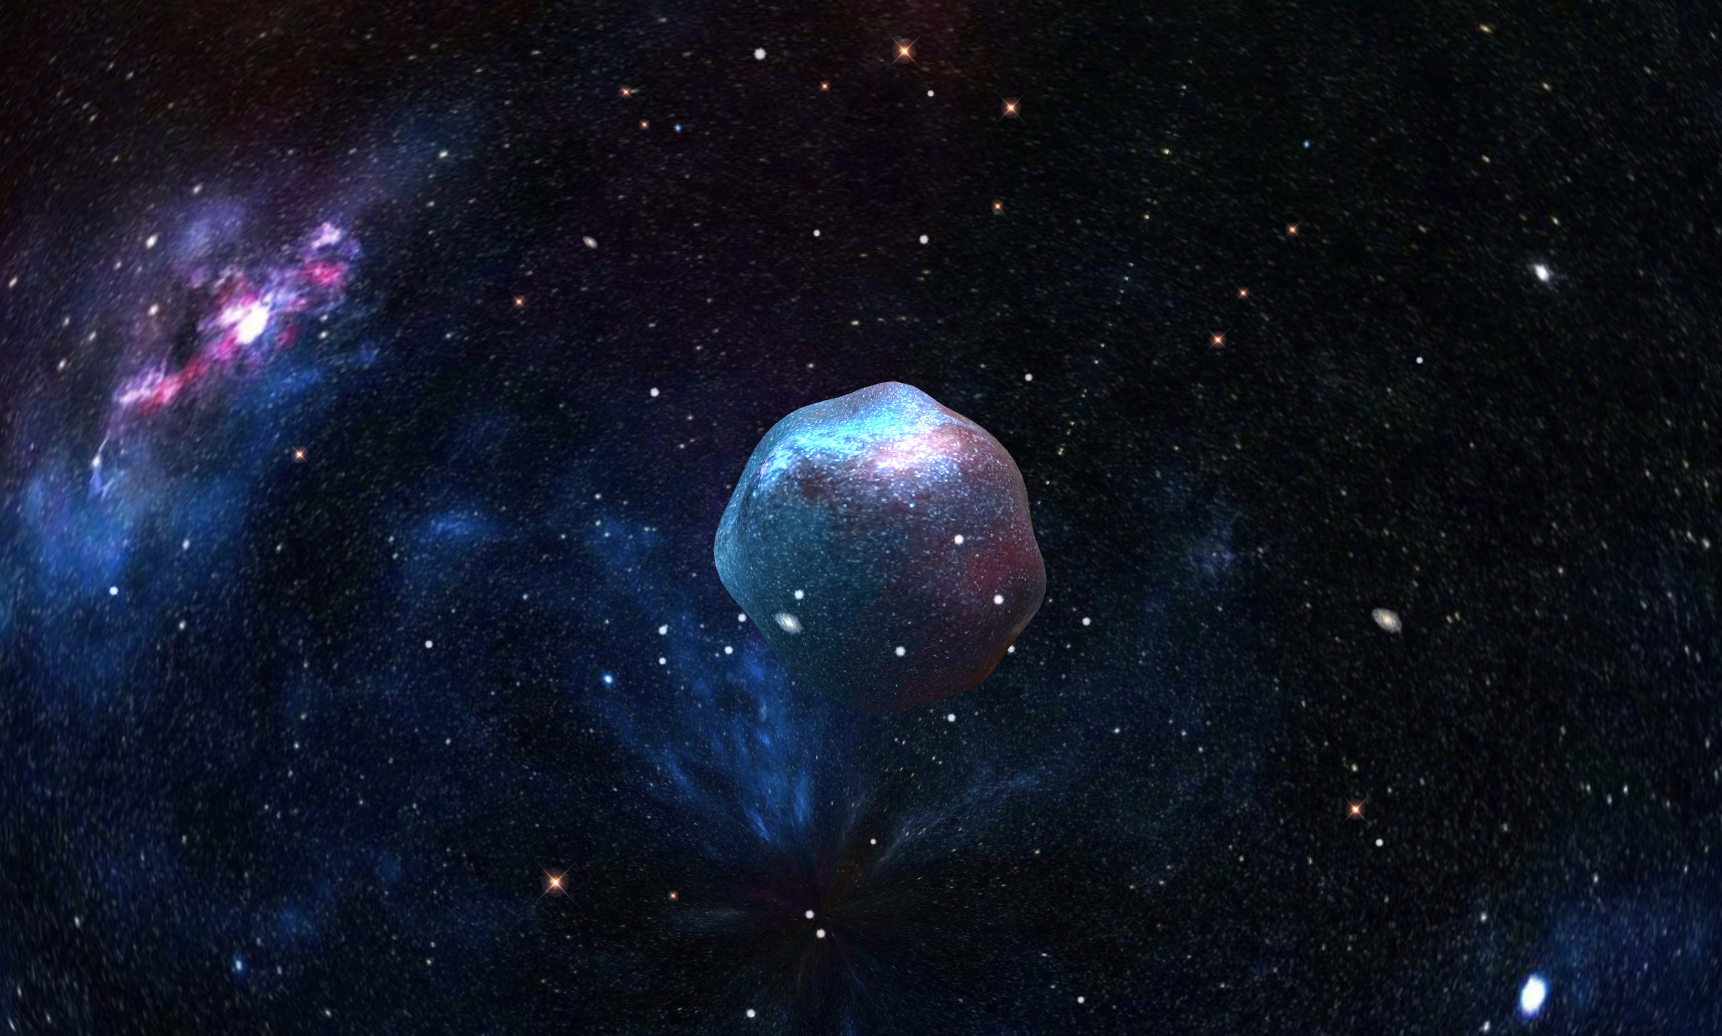
\includegraphics[width=9cm, keepaspectratio]{img/threejs.png}
  \caption{Escena creada con three.js}\label{fig:three}
\end{figure}


\section{HTML5} % título de sección (se muestra)
\label{sec:HTML5}
HTML es uno de lo pilares fundamentales de este proyecto ya que es uno de las tecnologías mas usadas para la creación de este proyecto.

HTML~\cite{HTML} es un lenguaje de marcado utilizado en el desarrollo del contenido web. Suele estar acompañado por otras tecnologías que la complementan, en cuanto a apariencia, CSS, no muy utilizada en este proyecto y en cuanto a funcionalidad, JavaScript, muy utilizada en este trabajo.

Una de las características de HTML es la utilización de marcas para etiquetar los distintos elementos del documento para luego mostrarlo en la web. Algunas de las etiquetas son: \begin{verbatim}<head>, <ul>, <p>, <span>.\end{verbatim} 

Estas etiquetas permiten al elemento tener una gran versatiliad, estructura lógica y facilidad a la hora de entenderlo. Dentro de estas podemos encontrar los atributos\footnote{\url{https://es.wikipedia.org/wiki/Atributo_HTM}} que son utilizados para controlar el comportamiento de dicha equiqueta.

Un ejemplo básico de un documento HTML puede ser el siguiente:

\begin{verbatim}
<!DOCTYPE html>
<html>
  <head>
    <meta charset="utf-8">
    <title>TFG Julian</title>
  </head>
  <body>
    <p>Hola mundo!</p>
  </body>
</html>
\end{verbatim}
Cuando hablamos de HTML es importante destacar el DOM, es la estructura de todos elementos del documento organizados en nodos, el conjunto de todos estos se denomina arbol de nodos. Gracias al DOM y al lenguaje JavaScript podremos acceder a los elementos para un libre utilización de ellos.


\begin{figure}[H]
  \centering
  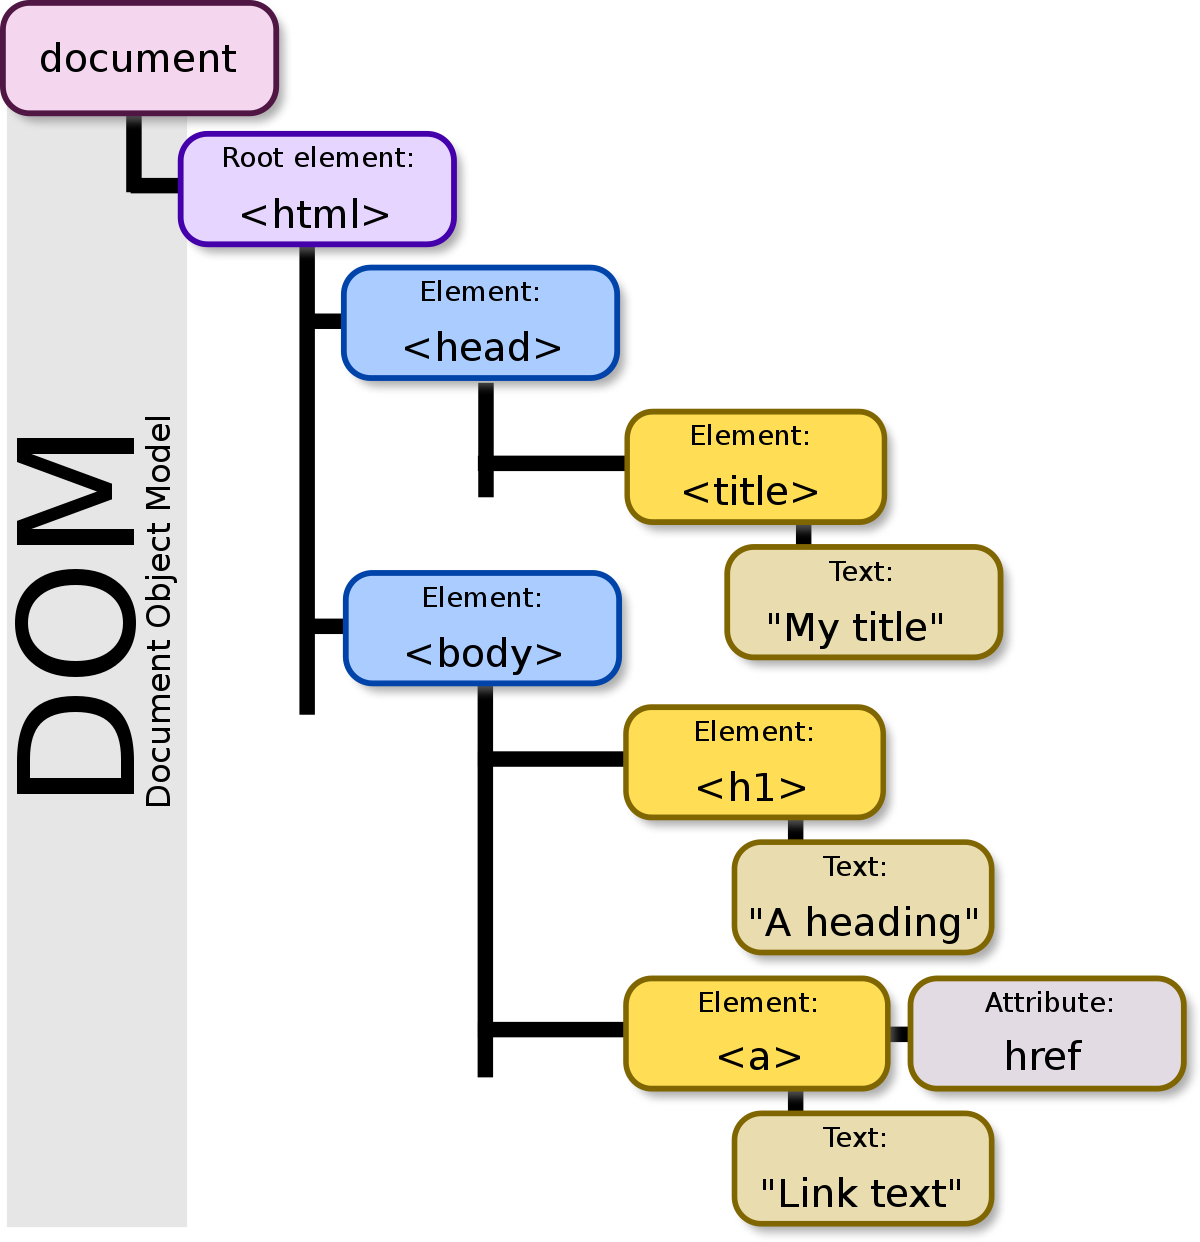
\includegraphics[width=9cm, keepaspectratio]{MemoriaTFG-JulianPerez/img/1200px-DOM-model.svg.png}
  \caption{Visualización gráfica del DOM}\label{html}
\end{figure}


Para terminar, destacar que ahora mismo HTML se ecuentra en su versión HTML5, publicada en 2014, donde se añadieron varias nuevas funcionalidades como la inclusión de nuevas etiquetas o la compatibilidad con varias APIS con Canvas o WebGL.
\section{JavaScript} % título de sección (se muestra)
\label{sec:JavaScript}

JavaScript(JS)~\cite{eloquent} es el lenguaje de programación que se complementa con el lenguaje anteriormente explicado, HTML. JS se suele utlizar para controlar comportamientos de la página web.

Para ampliar información sobre este, podemos decir que JavaScript es un lenguaje que permite la construcción de objetos basada en prototipos\footnote{\url{https://es.wikipedia.org/wiki/Programación_basada_en_prototipos}}, esto ayuda al programador ha crear objetos no mediante el uso de  instancias de clases sino mediante la clonación de objetos. La sintaxis de Javascript con la intención de no complicar mucho este, es muy parecida a otros lenguajes como Java y C++.

Centrandonos en las funcionalidades que ofrece este lenguaje, Javascript nos permite crear los comportamientos de los distintos elementos  HTML mediante el acceso al DOM, A continuación puedes ver un pequeño ejemplo de como realizar un hola mundo en JavaScript:


\begin{verbatim}
 <script>
  document.write("Hola Mundo");
</script>   
\end{verbatim}

Gracias a este lenguaje, puedes crear contenido de actualización dinámica con la creación de eventos, controlar multimedia o animar imágenes, por lo que HTML deja de ser un lenguaje estático.

JavaScript se utiliza principalmente del lado del cliente como parte del navegador web. Si hablamos del lado del servidor podemos hablar de Node.js\footnote{\url{https://nodejs.org/es/}}, se trata de un entorno  en tiempo de ejecucion basado en JS



\section{A-Frame} % título de sección (se muestra)
\label{sec:A-Frame}

A-frame~\cite{a} es la tecnología más importante de este proyecto, ya que es la base fundamental de este. A-frame es un framework creado para la construcción de experiencias en realidad virtual, basado en HTML, por lo que como hemos dicho antes, es un leguaje bastane sencillo e intuitivo. Una de las caracteristicas claves de A-frame es el framwork entidad-componente para three.js.

Esta tecnología fue desarrollada por el equipo de mozilla VR durante 2015. El objetivo principal de estos era permitir crear dichas escenas directamente en HTML sin conocer WebGL. A parte de esta, también usa otras tecnologías anteriormente explicadas como son WebXR y JavaScript.

Un ejemplo de creación de figuras en A-frame mediante HTML puede ser el siguiente:\begin{verbatim}
<html>
  <head>
    <script src="https://aframe.io/releases/1.2.0/aframe.min.js"></script>
  </head>
  <body>
    <a-scene>
      <a-box position="-1 0.5 -3" rotation="0 45 0" color="#4CC3D9"></a-box>
      <a-sphere position="0 1.25 -5" radius="1.25" color="#EF2D5E"></a-sphere>
      <a-cylinder position="1 0.75 -3" radius="0.5" height="1.5" color="#FFC65D"></a-cylinder>
      <a-plane position="0 0 -4" rotation="-90 0 0" width="4" height="4" color="#7BC8A4"></a-plane>
      <a-sky color="#ECECEC"></a-sky>
    </a-scene>
  </body>
</html>
\end{verbatim}

El resultado en la página web de este codigo, es el siguiente:

\begin{figure}[H]
  \centering
  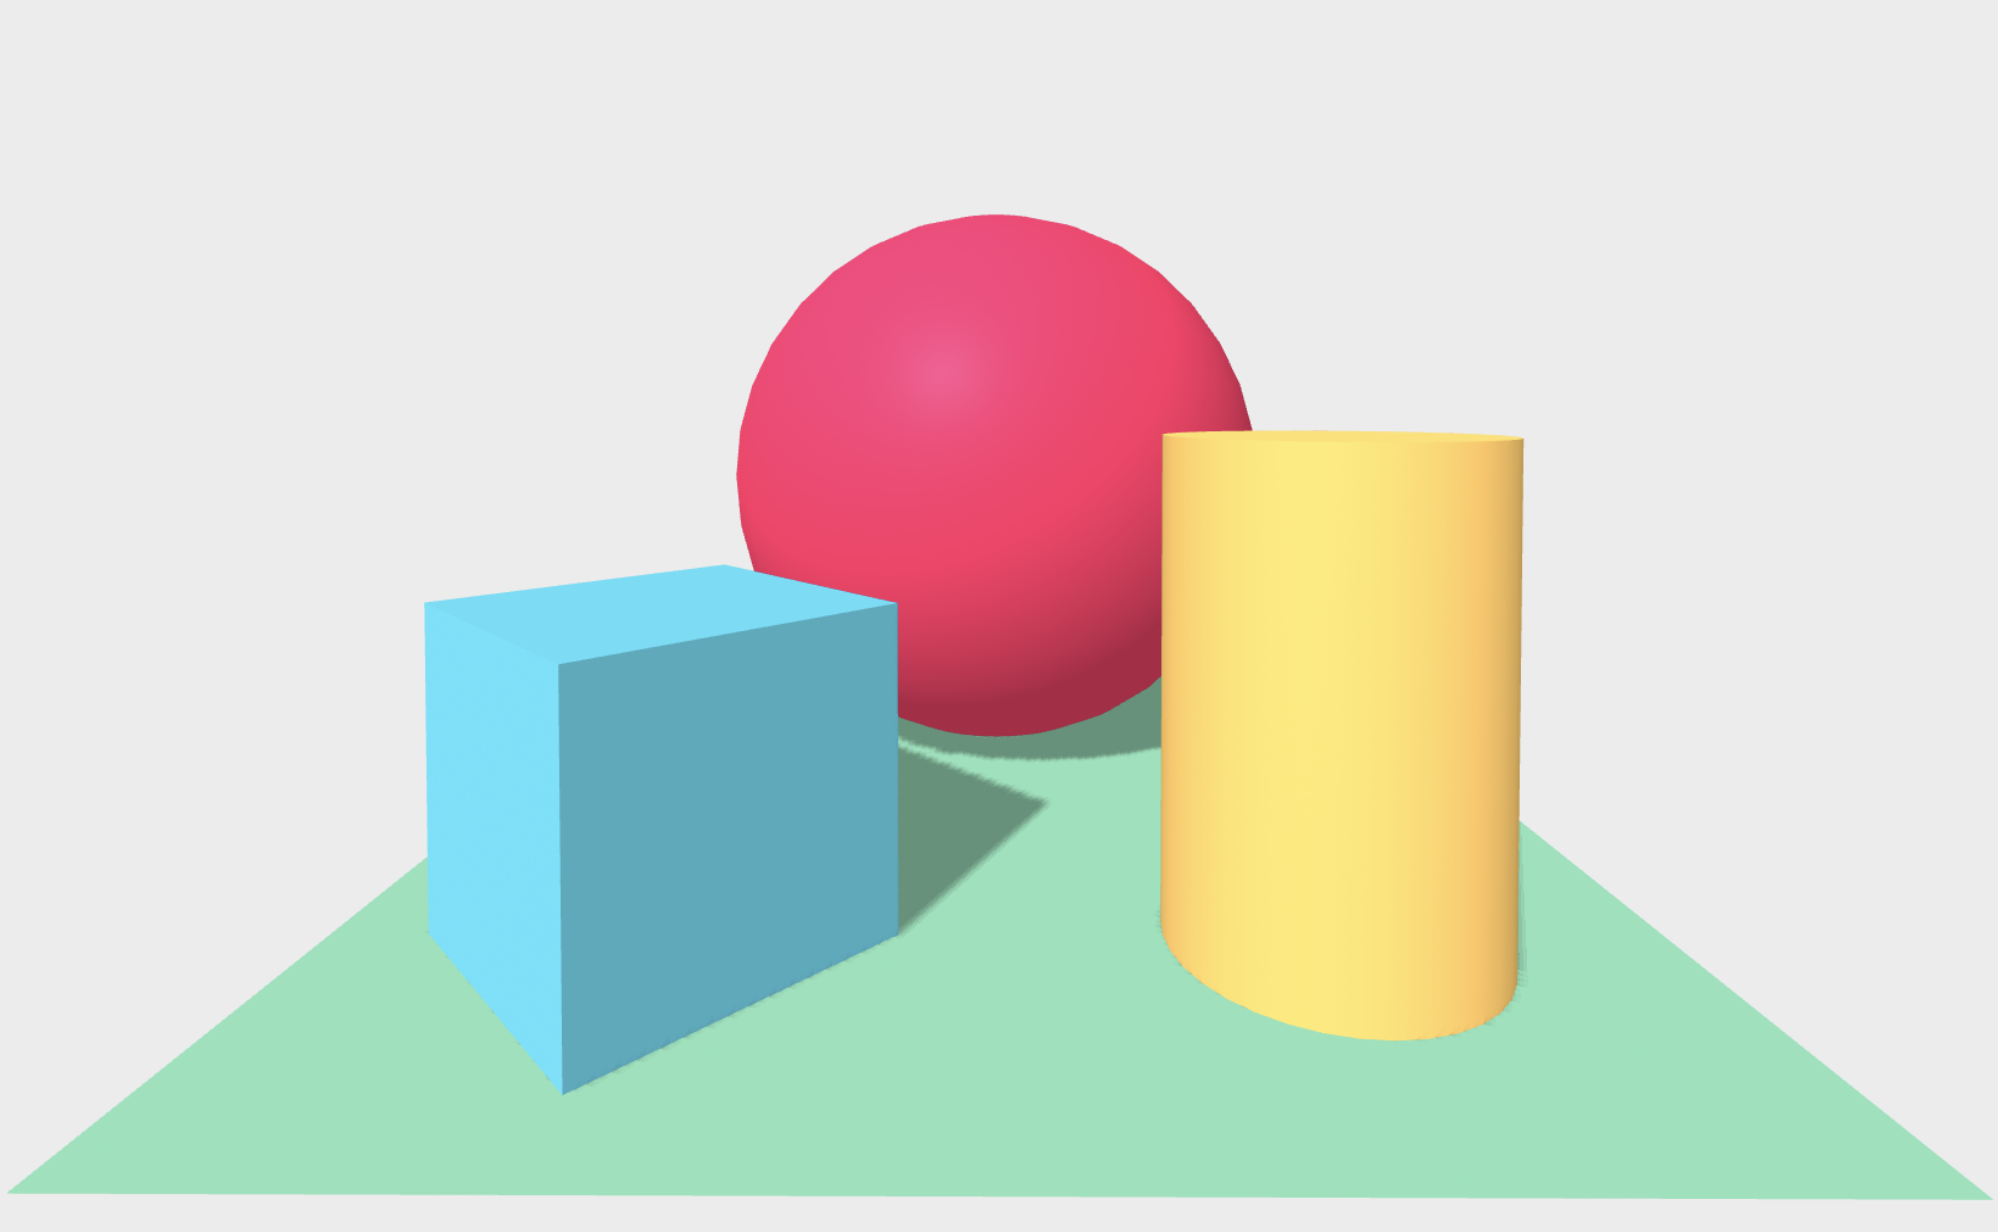
\includegraphics[width=12cm, keepaspectratio]{MemoriaTFG-JulianPerez/img/aframe.png}
  \caption{Escena básica A-Frame}\label{aframe}
\end{figure}

Explicando un poco mas sobre el codigo del escenario de ejemplo, podemos destacar: 

\begin{itemize}
    \item La inclusion de las dependencias de Aframe en el elemento Head, esto nos permite usar todos los elementos de esta tecnología.
    \item La creacion de las diferentes figuras mediante sus respectivas etiquetas.
    \item Modificación de ciertos aspectos de las figturas mediante los atributos.
\end{itemize}

Profundizando un poco más sobre la relación entidad-componente, Una entidad es el objeto en sí creado mediante HTML y el componente es el corportamiento que le podemos asginar a dicha figura, estos se realiza en el JavaScript. 

Estos componentes siguen una estructura estandarizada, algunos son elementos de dicha estructura son: schema, propiedas del componente, init, parte del componente que se ejectuta al iniciar el componente. La manera correcta de incluir un componente a la escena es añadirselo al elemento como si de un atributo se tratara.

 
\section{Github} % título de sección (se muestra)
\label{sec:GitHub}
GitHub~\cite{GITHUB} es una platafroma de almacenamiento y administración  de software, Este sistema está basado en el control de versiones \footnote{\url{https://es.wikipedia.org/wiki/Control_de_versiones}} y en Git \footnote{\url{https://git-scm.com}}.

Gracias al control de versiones, el desarrollador puede administrar y llevar un registro de cualquier modificación sobre el proyecto. Este sistema permite al desarrollador trabajar de una forma segura mediante las ramas. Las ramas te permiten duplicar el codigo fuente, donde puede hacer cambios sin afectar al proyecto "principal". Puedes fusionar las distintas ramas si lo deseas.

En cuanto a Git, se trata de un sistema de control de versiones, es decir te ayuda a controlar lo anterior explicado mediante el terminal del ordenador.

Tras esto, podemos explicar de una manera mas específica que es Github, este es una interfaz gráfica de Git el cual nos ofrece distintas funcionalidades como pueden ser, la creación de un usuario, la creación de distintos proyectos(repositorios) los cuales modificar desde la propia interfaz web, capacidad de trabajar en repositorios creados por otros desarrolladores mediante un fork\footnote{\url{https://es.wikipedia.org/wiki/Bifurcación_(desarrollo_de_software)}} o la modificación del mismo mediante un pull, creacion de un foro en los que los desarroladores pueden expresar dudas/problemas sobre el proyecto, etc.

Hoy en día según el 87\% de los desarrolladores utilizan GitHub, en mi caso ha sido la plataforma principal en la cual he ido utilizando para el desarrollo del proyecto.


\section{PyCharm} % título de sección (se muestra)
\label{sec:GitHub}
Se trata de un entorno de desarrollo integrado (IDE) que se utiliza para la programación, es un software creado por la compañia JetBrains~\cite{jetbrains}.

Este software es multiplataforma adaptado para Windows, macOS y Linux. Ha sido utilizado para la creación de este proyecto y por eso es una parte fundamental de esto.

Tiene infinidad de ventajas entre las que están:

\begin{itemize}
    \item Asistencia y análisis de codificación, con ayuda a la finalización del codigo, sintaxis y resaltado de errores.
    \item Navegación entre proyectos y ficheros.
    \item Acceso a la ejecución del codigo en el navegador mediante accesos directos.
\end{itemize}

Pycharm proporciona una API para que los desarrolladores puedan crear distintos plugins y de este modo se pueda crear codigo de manera más facil y eficiente.

\section{Latex} % título de sección (se muestra)
\label{sec:Latex}
LaTeX está basado en Tex\footnote{\url{https://es.wikipedia.org/wiki/TeX}}, programa destinado a la creación de documentos que contienen textos y fórmulas matemáticas. Este programa no es un editor de textos, si no, un procesador de macros.

LaTeX es un conjunto de macros para Text, cuyo objetivo principal es la alta composición tipográfica. Está orientando a la producción y creación de documentos científicos y se ha estandarizado para la creación de los mismos.

Esta tecnología nos presenta diversas ventajas entre las que se encuentran la faciliad de gestionar las referencias, bibliografias, etc, es un sistema multiplataforma, puedes componer fórmulas con calidad de imprenta o la capacidad de exportar el documento a PDF. La creación de dichos documentos puede ser al principio, un poco complicado si no se conoce la herramienta.

Se trata de un softwate libre bajo la licencia LPPL\footnote{\url{https://es.wikipedia.org/wiki/LaTeX_Project_Public_License}} 

Este sistema ha sido fundamental a la hora de crear este proyecto ya que esta memoria esta creada utilizando LaTeX.

\section{Gltfs} % título de sección (se muestra)
\label{sec:Gltfs}
Este formato de archivo tiene como objetivo principal escenas y modelos en 3D y esta basado en el foramto de texto sencillo para el intercambio de datos, JSON. Porpularmente se le describe como como el JPEG en 3D.

Este formato esta creado para una eficiente distribución de objetos y escenas en 3D, disminuyendo el tiempo de procesameinto en ejecución. Este formato se puede usar en aplicaciones que usan la tecnología anteriormente explicada, WebGl.

Es importante explicar este formato, ya que la aplicación que he creado te permite el manejo y  modificación de este formato en la aplicación.

\section{Otros} % título de sección (se muestra)
\label{sec:Otros}
En esta sección es importante destacar otros editores que trabajar en VR como son Blender, centrado en aspectos como la renderización, creación de gráficos en 3D o Unity centrado en creación del motror gráfico en videojuegos. Ya que mi proyecto es un pequeño paso para la creación de un gran editor.

Existen otros editores como son, OpenCat o AutoCat.

%%%%%%%%%%%%%%%%%%%%%%%%%%%%%%%%%%%%%%%%%%%%%%%%%%%%%%%%%%%%%%%%%%%%%%%%%%%%%%%%
%%%%%%%%%%%%%%%%%%%%%%%%%%%%%%%%%%%%%%%%%%%%%%%%%%%%%%%%%%%%%%%%%%%%%%%%%%%%%%%%
% ESTADO DEL ARTE %
%%%%%%%%%%%%%%%%%%%%%%%%%%%%%%%%%%%%%%%%%%%%%%%%%%%%%%%%%%%%%%%%%%%%%%%%%%%%%%%%

\cleardoublepage
\chapter{Desarrollo del proyecto}
\label{chap:Desarrollo del proyecto}
Para poder hablar del desarrollo tenemos que comenzar explicando la metodología scrum~\cite{proyectos} ya que ha sido la utilizada para la creación de este proyecto.

Scrum es un metodología que esta centrada en el desarrollo ágil\footnote{\url{https://es.ryte.com/wiki/Desarrollo_Ágil_de_Software}}  de software, aunque he realizado el proyecto de manera individual esta metodología se suele aplica de manera colectiva con la participacion en equipo con el objetivo de obtener el mejor resultado posible.

En cuanto a la historia de esta metodología, oficialmente surgio en 1995 presentado por Ken Schwaber y Jeff Sutherland mediante "scrum DEvelopment Process". Aunque esta fuera la fecha "oficial" este modelo ya se habia dejado ver en los años 80.

En Scrum se pueden diferenciar distintos roles, Scrum Master, Product ownery el equipo. El rol de scrum Master en este caso esta representado por el tutor del proyecto cuya funcion es facilitar y ayudar a gestionar el trabajo. En este caso el product owner no tiene un papel importante y respecto al team esta representapo por mi, el alumno que realiza este proyecto y su función es el desarrollo y la entrega de las distintas tareas organizadas en cada sprint.

Sobre los sprint, se tratan de distintos periodos de tiempo en el cual el equipo, en este caso yo, me centro en la realización de las tareas marcadas. Estos sprint se iniciaban con un reunión Scrum Master - Team en la cual se fijaba unos objetivos y se marcaban los pasoos a seguir para la consecución de dichos objetivos. Tras un tiempo trabajando en el sprint se emplaza otra nueva reunión en la cual se comparte la tarea terminada y los problemas que han ido surgiendo durante esta.En esta misma reunión el equipo prepara un version funcional de la aplicación o tarea y se marcan los siguientes pasos, el comienzo de un nuevo sprint. 

Podemos ver más en detalle el proceso en la siguiente imagen:
\begin{figure}[H]
  \centering
  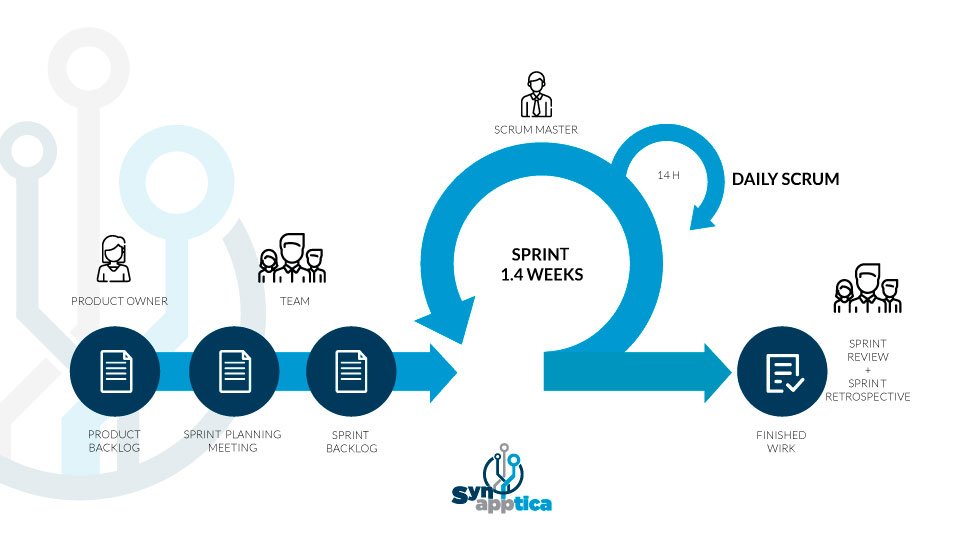
\includegraphics[width=12cm, keepaspectratio]{MemoriaTFG-JulianPerez/img/Scrum.jpg}
  \caption{Estructura metodología Scrum}\label{scrum}
\end{figure}

%%%%%%%%%%%%%%%%%%%%%%%%%%%%%%%%%%%%%%%%%%%%%%%%%%%%%%%%%%%%%%%%%%%%%%%%%%%%%%%%
%%%%%%%%%%%%%%%%%%%%%%%%%%%%%%%%%%%%%%%%%%%%%%%%%%%%%%%%%%%%%%%%%%%%%%%%%%%%%%%%
% DISEÑO E IMPLEMENTACIÓN %
%%%%%%%%%%%%%%%%%%%%%%%%%%%%%%%%%%%%%%%%%%%%%%%%%%%%%%%%%%%%%%%%%%%%%%%%%%%%%%%%

\cleardoublepage
\chapter{Resultados}

Aquí viene todo lo que has hecho tú (tecnológicamente). 
Puedes entrar hasta el detalle. 
Es la parte más importante de la memoria, porque describe lo que has hecho tú.
Eso sí, normalmente aconsejo no poner código, sino diagramas.

\section{Arquitectura general} 
\label{sec:arquitectura}

Si tu proyecto es un software, siempre es bueno poner la arquitectura (que es cómo se estructura tu programa a ``vista de pájaro'').

Por ejemplo, puedes verlo en la figura~\ref{fig:arquitectura}.
\LaTeX \ pone las figuras donde mejor cuadran. 
Y eso quiere decir que quizás no lo haga donde lo hemos puesto\ldots
Eso no es malo.
A veces queda un poco raro, pero es la filosofía de \LaTeX: tú al contenido, que yo me encargo de la maquetación.

\begin{figure}
  \centering
  \includegraphics[width=9cm, keepaspectratio]{img/arquitectura.png}
  \caption{Estructura del parser básico.}\label{fig:arquitectura}
\end{figure}

\begin{figure}
    \centering
    \includegraphics[bb=0 0 800 600, width=12cm, keepaspectratio]{img/foro1}
    \caption{Página con enlaces a hilos}\label{fig:_arquitectura}
\end{figure}

 
Recuerda que toda figura que añadas a tu memoria debe ser explicada.
Sí, aunque te parezca evidente lo que se ve en la figura~\ref{fig:arquitectura}, la figura en sí solamente es un apoyo a tu texto.
Así que explica lo que se ve en la figura, haciendo referencia a la misma tal y como ves aquí.
Por ejemplo: En la figura~\ref{fig:arquitectura} se puede ver que la estructura del \emph{parser} básico, que consta de seis componentes diferentes: los datos se obtienen de la red, y según el tipo de dato, se pasará a un \emph{parser} específico y bla, bla, bla\ldots

Si utilizas una base de datos, no te olvides de incluir también un diagrama de entidad-relación.



%%%%%%%%%%%%%%%%%%%%%%%%%%%%%%%%%%%%%%%%%%%%%%%%%%%%%%%%%%%%%%%%%%%%%%%%%%%%%%%%
%%%%%%%%%%%%%%%%%%%%%%%%%%%%%%%%%%%%%%%%%%%%%%%%%%%%%%%%%%%%%%%%%%%%%%%%%%%%%%%%
% CONCLUSIONES %
%%%%%%%%%%%%%%%%%%%%%%%%%%%%%%%%%%%%%%%%%%%%%%%%%%%%%%%%%%%%%%%%%%%%%%%%%%%%%%%%

\cleardoublepage
\chapter{Conclusiones}
\label{chap:conclusiones}


\section{Consecución de objetivos}
\label{sec:consecucion-objetivos}

Esta sección es la sección espejo de las dos primeras del capítulo de objetivos, donde se planteaba el objetivo general y se elaboraban los específicos.

Es aquí donde hay que debatir qué se ha conseguido y qué no. 
Cuando algo no se ha conseguido, se ha de justificar, en términos de qué problemas se han encontrado y qué medidas se han tomado para mitigar esos problemas.

Y si has llegado hasta aquí, siempre es bueno pasarle el corrector ortográfico, que las erratas quedan fatal en la memoria final.
Para eso, en Linux tenemos aspell, que se ejecuta de la siguiente manera desde la línea de \emph{shell}:

\begin{verbatim}
  aspell --lang=es_ES -c memoria.tex
\end{verbatim}

\section{Aplicación de lo aprendido}
\label{sec:aplicacion}

Aquí viene lo que has aprendido durante el Grado/Máster y que has aplicado en el TFG/TFM. Una buena idea es poner las asignaturas más relacionadas y comentar en un párrafo los conocimientos y habilidades puestos en práctica.

\begin{enumerate}
  \item a
  \item b
\end{enumerate}


\section{Lecciones aprendidas}
\label{sec:lecciones_aprendidas}

Aquí viene lo que has aprendido en el Trabajo Fin de Grado/Máster.

\begin{enumerate}
  \item Aquí viene uno.
  \item Aquí viene otro.
\end{enumerate}


\section{Trabajos futuros}
\label{sec:trabajos_futuros}

Ningún proyecto ni software se termina, así que aquí vienen ideas y funcionalidades que estaría bien tener implementadas en el futuro.

Es un apartado que sirve para dar ideas de cara a futuros TFGs/TFMs.


%%%%%%%%%%%%%%%%%%%%%%%%%%%%%%%%%%%%%%%%%%%%%%%%%%%%%%%%%%%%%%%%%%%%%%%%%%%%%%%%
%%%%%%%%%%%%%%%%%%%%%%%%%%%%%%%%%%%%%%%%%%%%%%%%%%%%%%%%%%%%%%%%%%%%%%%%%%%%%%%%
% APÉNDICE(S) %
%%%%%%%%%%%%%%%%%%%%%%%%%%%%%%%%%%%%%%%%%%%%%%%%%%%%%%%%%%%%%%%%%%%%%%%%%%%%%%%%

\cleardoublepage
\appendix
\chapter{Manual de usuario}
\label{app:manual}

Esto es un apéndice.
Si has creado una aplicación, siempre viene bien tener un manual de usuario.
Pues ponlo aquí.

%%%%%%%%%%%%%%%%%%%%%%%%%%%%%%%%%%%%%%%%%%%%%%%%%%%%%%%%%%%%%%%%%%%%%%%%%%%%%%%%
%%%%%%%%%%%%%%%%%%%%%%%%%%%%%%%%%%%%%%%%%%%%%%%%%%%%%%%%%%%%%%%%%%%%%%%%%%%%%%%%
% BIBLIOGRAFIA %
%%%%%%%%%%%%%%%%%%%%%%%%%%%%%%%%%%%%%%%%%%%%%%%%%%%%%%%%%%%%%%%%%%%%%%%%%%%%%%%%

\cleardoublepage

% Las siguientes dos instrucciones es todo lo que necesitas
% para incluir las citas en la memoria
\bibliographystyle{abbrv}
\bibliography{memoria}  % memoria.bib es el nombre del fichero que contiene
% las referencias bibliográficas. Abre ese fichero y mira el formato que tiene,
% que se conoce como BibTeX. Hay muchos sitios que exportan referencias en
% formato BibTeX. Prueba a buscar en http://scholar.google.com por referencias
% y verás que lo puedes hacer de manera sencilla.
% Más información: 
% http://texblog.org/2014/04/22/using-google-scholar-to-download-bibtex-citations/

\end{document}
